\section{Methodology}\label{sec:method}


\subsection{Model Architecture}

The overall pipeline of EMMA is depicted in Figure~\ref{fig:methods} (a). 
Our model's conditions encompass two aspects. One is the textual feature, and the other is the customized image features, such as visual clip features or facial embeddings.\\
In EMMA, we inject text features through Perceiver Resampler blocks proposed by ELLA~\cite{hu2024ella} as shown in Figure~\ref{fig:methods} (b). 
The image features are perceived by our newly proposed module named Assemblable Gated Perceiver Resampler as shown in Figure~\ref{fig:methods} (c).

To be more specific, we categorize EMMA into three main components and describe them in detail. 

\textbf{Text Encoder:} T5~\cite{chung2024scaling} is equipped to understand rich textual content. Prior research has shown that T5 is adept at extracting textual features, which makes it well-suited for supplying textual features to downstream tasks.

\textbf{Image Generator:} In the realm of image generation, numerous researchers and practitioners have fine-tuned various models on a clip-specific basis, aligning with their specific goals and data types. We strive for our final network to ensure the generalization of features, thereby maximizing the use of the high-quality models prevalent in the community.

\textbf{Multi-modal Feature Connector:} The network architecture is depicted in Figure~\ref{fig:methods}. Drawing inspiration from Flamingo~\cite{alayrac2022flamingo} and ELLA, the connector consists of two alternating stacked network modules: the Perceiver Resampler and the Assemblable Gated Perceiver Resampler. 
The Perceiver Resampler is primarily tasked with integrating textual information, while the Assemblable Gated Perceiver Resampler is designed to incorporate additional information. These network modules use an attention mechanism to assimilate multimodal information into the learnable token embeddings, which are then supplied to the U-net as conditions.
We give the definitions of these blocks as follows. The connector contains $K$ learnable tokens, denoted by $Latent$. Time embeddings, textual features, and additional conditions are represented by $t$, $T$, and $C$, respectively.

The Perceiver Resampler block can be divided into two parts:

\begin{equation}
    L = L + \mathtt{TimeAwareAttn}(L, T, t),
\end{equation}
\begin{equation}
    L = L + \mathtt{TimeAwareFFN}(L, t).
\end{equation}

Here, $\mathtt{TimeAwareAttn}$ and $\mathtt{TimeAwareFFN}$ are custom attention and feedforward neural network (FFN) modules that utilize AdaLN to integrate time embeddings into the inputs. The advantages of this approach have been demonstrated by ELLA.

The Assemblable Gated Perceiver Resampler is formulated similarly:

\begin{equation}
    L = L + AttnGate \cdot \mathtt{TimeAwareAttn}(L, C, t),
\end{equation}
\begin{equation}
    L = L + FFNGate \cdot \mathtt{TimeAwareFFN}(L, t).
\end{equation}

In these equations, $AttnGate$ and $FFNGate$ are two sets of gates that regulate the feature integration. Their definitions are as follows:

\begin{equation}
    AttnGate = \lambda \cdot \mathtt{Linear}(L) \cdot A
\end{equation}
\begin{equation}
    FFNGate = \lambda \cdot \mathtt{Linear}(L) \cdot F
\end{equation}

Here, $\lambda$ is the gate scale, a fixed hyperparameter, and $A$ and $F$ are global gates. $\mathtt{Linear}(L)$ are separable gates. 





\begin{figure}[t]
    \centering
    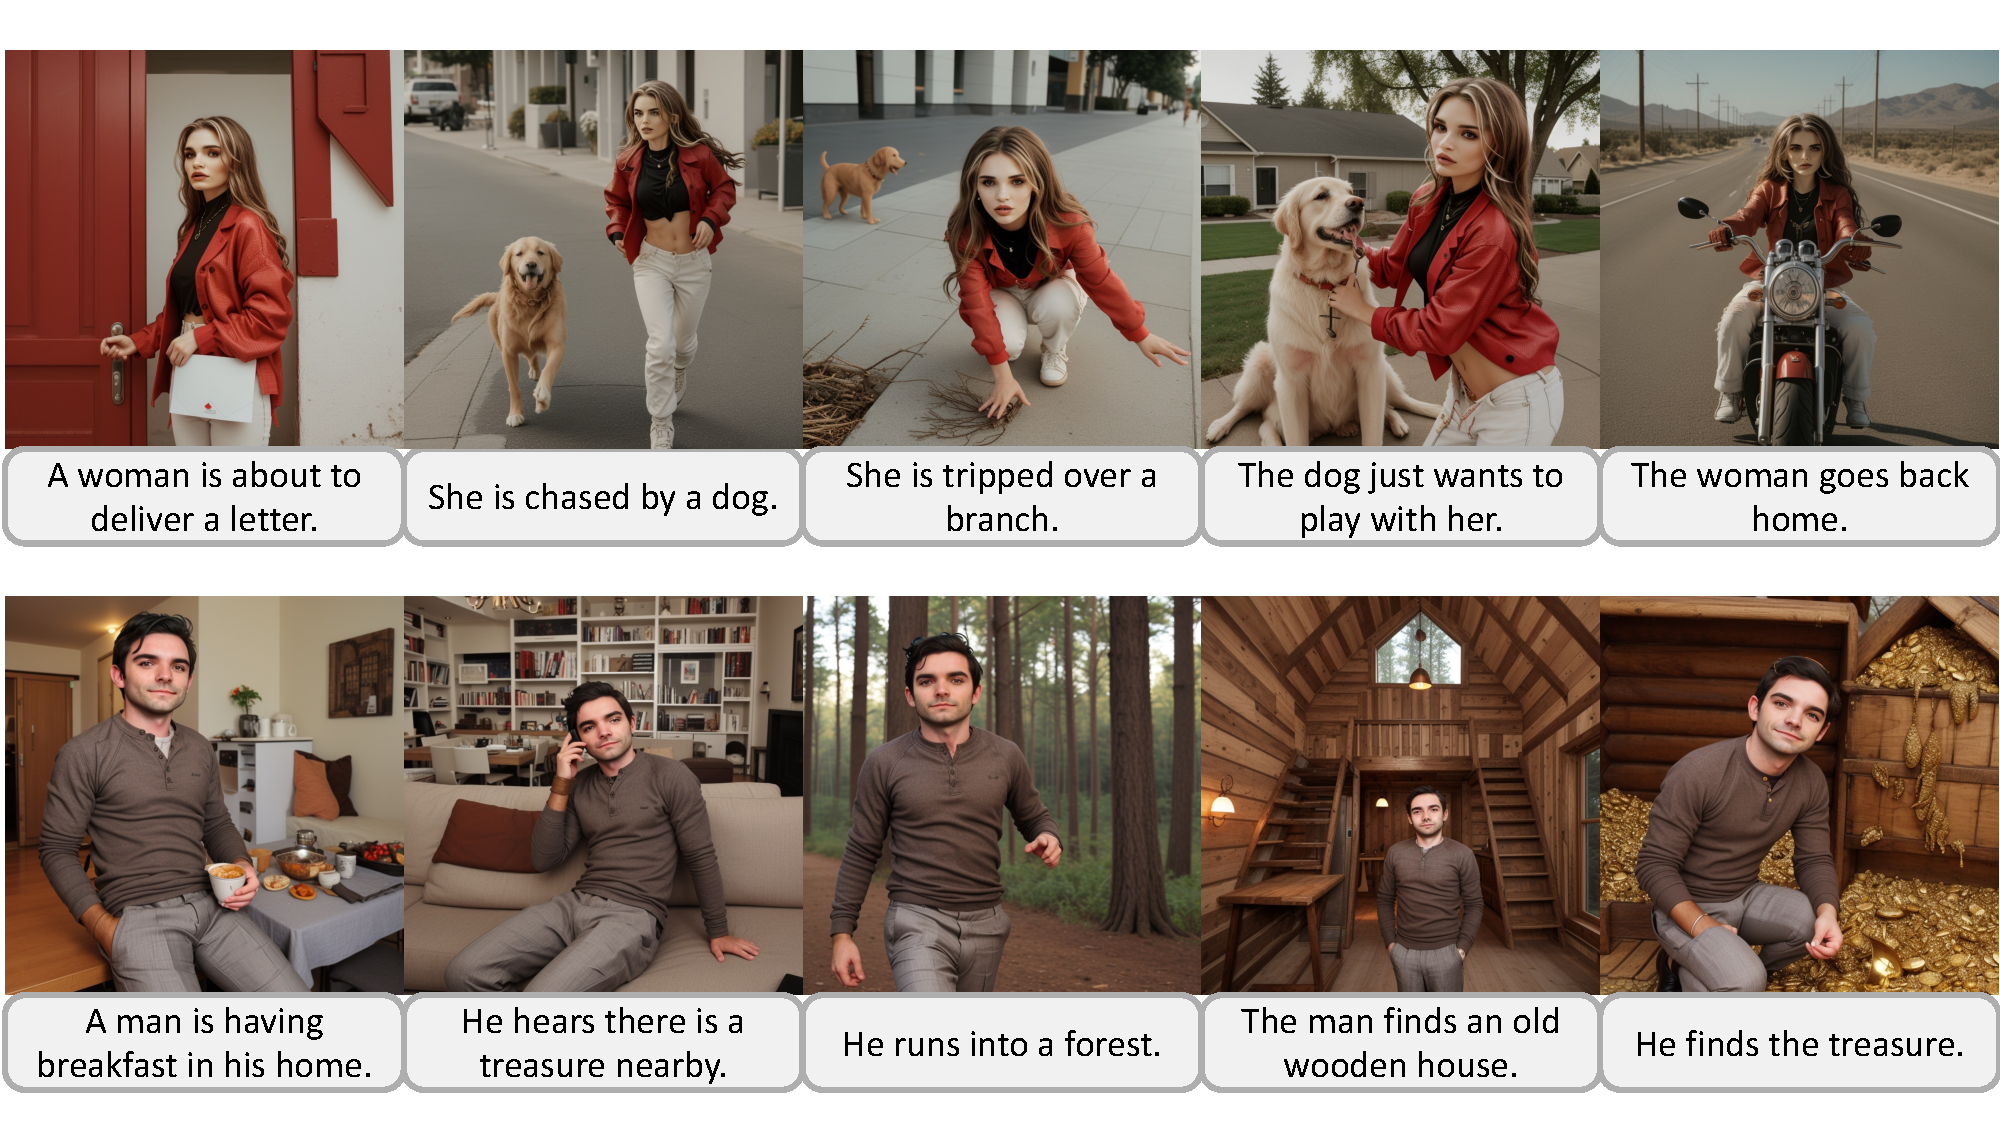
\includegraphics[width=0.9\textwidth]{images/Story_diffusion.pdf}
    \caption{Images generated by our EMMA with portrait conditions. Two sets of images are generated for two separate stories. The first set of images is about a mailing woman chased by a dog. The second set of images is about a man finding treasures.}
    \label{fig:story_diffusion}
\end{figure}

\subsection{Image Generation with Multiple Conditions}

\textbf{Developing Text-to-Image Capability.} Through ELLA's training paradigm, we have developed a text-to-image model endowed with robust text-to-image capabilities. As illustrated in the first row of Figure~\ref{fig:final_visualization}, ELLA can generate images that strictly adhere to instructions, which forms the foundation for EMMA's multi-modal guidance.

\textbf{Selective Modular Feature Training.} To bolster the stability and enhance the final performance of the training process, we have integrated several innovative design elements into the network architecture. For example, the alternating structure between the Perceiver Resampler and the Assemblable Gated Perceiver Resampler is designed to limit the feature space of the network's intermediate layers. This prevents image information from imparting excessive prior knowledge that might compromise the text's control and disrupt the final generation outcomes. The Assemblable Gated Perceiver Resampler includes separated gates that enable the incorporation of additional features into a few trainable embeddings. 

\textbf{Assembling Modules for Multi-Condition Image Generation.} After establishing strong models for each individual condition, we have devised an innovative approach that enables the model to amalgamate existing modules and produce images conditioned by multiple factors. As depicted in the figure, we integrate the Assemblable Gated Perceiver Resampler. Without additional training, the model can synthesize all input conditions and generate novel outputs. This demonstrates the potential for image generation without relying on a pre-existing training dataset.

The process can be mathematically expressed as:
\begin{equation}
    L = L + \sum_{i} \lambda_i \cdot \mathtt{AttnGate}_i \cdot \mathtt{TimeAwareAttn}(L, C_i, t_i),
\end{equation}

\begin{equation}
    L = L + \sum_{i} \lambda_i \cdot \mathtt{FFNGate}_i \cdot \mathtt{TimeAwareFFN}(L, t_i).
\end{equation}

In this manner, various conditions can be applied to the image generation process without the need for further training.






